%%%%%%%%%%%%%%%%%%%%%%%%%%%%%%%%%%%%%%%%%
% Class Notes Template
% LaTeX Template
% By: Ryan Grove
%%%%%%%%%%%%%%%%%%%%%%%%%%%%%%%%%%%%%%%%%

%----------------------------------------------------------------------------------------
%	PACKAGES AND OTHER DOCUMENT CONFIGURATIONS
%----------------------------------------------------------------------------------------

\documentclass[paper=a4, fontsize=11pt]{scrartcl} % A4 paper and 11pt font size

\usepackage[T1]{fontenc} % Use 8-bit encoding that has 256 glyphs
\usepackage{fourier} % Use the Adobe Utopia font for the document - comment this line to return to the LaTeX default
\usepackage[english]{babel} % English language/hyphenation
\usepackage{amsmath,amsfonts,amsthm} % Math packages

\usepackage{lipsum} % Used for inserting dummy 'Lorem ipsum' text into the template

\usepackage{sectsty} % Allows customizing section commands
\allsectionsfont{\centering \normalfont\scshape} % Make all sections centered, the default font and small caps

\usepackage{fancyhdr} % Custom headers and footers
\pagestyle{fancyplain} % Makes all pages in the document conform to the custom headers and footers
\fancyhead{} % No page header - if you want one, create it in the same way as the footers below
\fancyfoot[L]{} % Empty left footer
\fancyfoot[C]{} % Empty center footer
%\fancyfoot[R]{\thepage} % Page numbering for right footer
\renewcommand{\headrulewidth}{0pt} % Remove header underlines
\renewcommand{\footrulewidth}{0pt} % Remove footer underlines
\setlength{\headheight}{13.6pt} % Customize the height of the header

\numberwithin{equation}{section} % Number equations within sections (i.e. 1.1, 1.2, 2.1, 2.2 instead of 1, 2, 3, 4)
\numberwithin{figure}{section} % Number figures within sections (i.e. 1.1, 1.2, 2.1, 2.2 instead of 1, 2, 3, 4)
\numberwithin{table}{section} % Number tables within sections (i.e. 1.1, 1.2, 2.1, 2.2 instead of 1, 2, 3, 4)

\setlength\parindent{0pt} % Removes all indentation from paragraphs - comment this line for an assignment with lots of text

\usepackage{lastpage}
\usepackage{fancyhdr}
\cfoot{\thepage\ of \pageref{LastPage}}

\def\v{\hbox{$\mathbf v$}}
\def\w{\hbox{$\mathbf w$}}
\def\u{\hbox{$\mathbf u$}}
\def\x{\hbox{$\textbf{x}$}}
\def\z{\hbox{$\mathbf z$}}
\def\a{\hbox{$\mathbf a$}}
\def\b{\hbox{$\mathbf b$}}
\def\L{\hbox{$\mathcal L$}}
\def\C{\hbox{$\mathbb C$}}
\def\B{\hbox{$\mathcal B$}}
\def\R{\hbox{$\mathbb R$}}
\def\X{\hbox{$\underline X$}}
\def\Q{\hbox{$\mathbb Q$}}
\def\R{\hbox{$\mathbb R$}}
\def\N{\hbox{$\mathbb N$}}
\def\C{\hbox{$\mathbb C$}}
\def\0{\hbox{$\mathbf 0$}}
\def\Y{\hbox{$\underline Y$}}
\def\a{\hbox{$\mathbf a$}}
\def\u{\hbox{$\mathbf u$}}
\def\w{\hbox{$\mathbf w$}}
\def\y{\hbox{$\mathbf y$}}
\def\X{\hbox{$\underline X$}}
\def\dd{\hbox{$\partial $}}
\def\B{\hbox{$\mathcal B$}}
\def\F{\hbox{$\mathcal F$}}
\def\L{\hbox{$\mathcal L$}}
\def\M{\hbox{$\mathcal M$}}
\def\D{\hbox{$\mathscr {D}$}}
\def\RR{\hbox{$\mathscr{R}$}}
\def\I{\hbox{$\mathcal I$}}

\usepackage{amssymb}
%\theoremstyle{plain}
\usepackage[margin = .75in]{geometry}
\newtheorem{claim}{Claim}
\newtheorem{theorem}{Theorem}[section]
\newtheorem{lemma}[theorem]{Lemma}
\newtheorem{proposition}[theorem]{Proposition}
\newtheorem{corollary}[theorem]{Corollary}
\newtheorem{problem}[theorem]{Problem}
%\theoremstyle{definition}
\newtheorem{definition}[theorem]{Definition}
%\theoremstyle{remark}
\newtheorem{remark}[theorem]{Remark}
\newtheorem{remarks}[theorem]{Remarks}
\newtheorem{example}[theorem]{Example}
\newcommand{\ds}{\displaystyle}
\newcommand{\ZZ}{\mathbb{Z}}
\newcommand{\QQ}{\mathbb{Q}}
\newcommand{\e}{\varepsilon}
\newcommand{\bbf}{\textbf}
\newcommand{\p}{\parallel}
\usepackage{color}
\newcommand{\field}[1]{\mathbb{#1}}
\usepackage{amsmath}
\usepackage{amsthm}
\usepackage{amssymb}
\usepackage{mathrsfs}
\usepackage{cancel}
\usepackage{upgreek}
\usepackage{graphicx}
\usepackage{multirow}
\usepackage{setspace}
\usepackage{url}
\usepackage{subfigure}
\usepackage{enumerate}
\usepackage{cases}
\usepackage{mathrsfs}
\usepackage{rotating}

%----------------------------------------------------------------------------------------
%	TITLE SECTION
%----------------------------------------------------------------------------------------

\newcommand{\horrule}[1]{\rule{\linewidth}{#1}} % Create horizontal rule command with 1 argument of height

\title{	
\normalfont \normalsize 
\textsc{Ryan Grove, Clemson University, MATH1080 - 9} \\ [25pt] % Your name, university, class
\horrule{0.5pt} \\[0.4cm] % Thin top horizontal rule
\huge Section 8.1: Arc Length \\ % The assignment title
\horrule{2pt} \\[0.5cm] % Thick bottom horizontal rule
}

\author{Date:} % The due date

\date{\normalsize February 15, 2016} % A custom date

\begin{document}

\maketitle % Print the title

\begin{flushleft}
\begin{tabular}{l l}
Name: \rule{3.2in}{.01cm}  & {}%Table number: \rule{1in}{.01cm}\\
\end{tabular}
\end{flushleft}

%----------------------------------------------------------------------------------------
%	Lecture
%----------------------------------------------------------------------------------------

\section*{\textbf{Lecture:}}

\[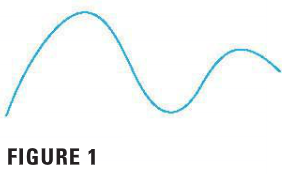
\includegraphics[scale=0.45]{8-1pic1.png}\]

What do we mean by the length of a curve? We might think of fitting a piece of string to the curve in Figure 1 and then measuring the string against a ruler. But that might be difficult to do with much accuracy if we have a complicated curve. We need a precise definition for the length of an arc (\textit{portion})of a curve, in the same spirit as the definitions we developed for the concepts of area and volume.\\
\indent

Suppose that a curve $C$ is defined by the equation $y=f(x)$, where $f$ is continuous and $a\leq x \leq b$. We obtain an approximation to $C$ by dividing the interval $[a,b]$ into $n$ subintervals with endpoints $x_0, x_1,\ldots,x_n$ and equal width $\Delta x$. If $y_i=f(x_i)$, then the point $P_i(x_i,y_i)$ lies on $C$ and the line segments connecting vertices $P_0,P_1,\ldots,P_n$ illustrated below, together form an approximation to $C$.

\[\hspace{2in} 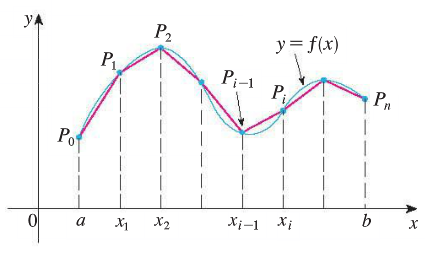
\includegraphics[scale=0.45]{8-1pic2.png} \hspace{2in} (1)\]

The length of $C$ is approximately the length of these line segments and we observe that the approximation gets better as we let $n$ increase. Therefore, we define the \underline{\hspace{1in}} $L$ of the curve $C$ with equation $y=f(x)$, $a\leq x\leq b$, as the limit of the combined lengths of these inscribed line segments (if the limit exists)

\[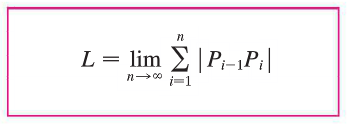
\includegraphics[scale=0.45]{8-1pic3.png}\]

This definition of arc length is not very convenient for computational purposes, but we can derive an integral formula for $L$ (arc length) in the case where $f$ has a continuous derivative.\\
\indent

If we let $\Delta y_i = y_i - y_{i-1}$, then the length of the $i^{\text{th}}$ line segment $\overline{P_{i-1}P_i}$ is:\\

\[|P_{i-1}P_i| = \ds\sqrt{(x_i-x_{i-1})^2 + (y_i-y_{i-1})^2} = \ds\sqrt{(\Delta x)^2 + (\Delta y_i)^2}\]

By applying the Mean Value Theorem to $f$ on the interval $[x_{i-1},x_i]$, we find that there is a number $x_i^*$ between $x_{i-1}$ and $x_i$ such that
\begin{align*}
f(x_i) - f(x_{i-1}) &= f'(x_i^*)(x_i-x_{i-1})\\
\implies \hspace{1in} \Delta y_i &= f'(x_i^*)\Delta x\\
\end{align*}

Thus we have,\\
\indent

\hspace{1in} $|P_{i-1}P_i| =$\\
\indent\\
\indent\\
\indent\\
\indent\\
\indent\\
\indent\\

Therefore, by definition (1),\\

\[L = \hspace{4.5in}\]
\indent

Thus we have proved the following theorem:\\
\indent\\

\fbox{
  \parbox{\textwidth}{
  \vspace{5pt} \textbf{The Arc Length Formula:} If $f'$ is continuous on $[a,b]$, then the length of the curve $y=f(x), a\leq x\leq b$, is
  \[L=\hspace{2.5in}\]
  
  or similarly using Leibniz notation,
  \[L = \ds\int_a^b\ds\sqrt{1+\left(\ds\frac{dy}{dx}\right)^2}\text{ }dx\]
  }}
  \indent\\
  \indent
  
  \underline{Note}: If a curve has the equation $x=g(y), c\leq y\leq d$, and $g'(y)$ is continuous, then by interchangin the roles of $x$ and $y$ above, we obtain the following formula for its length:\\
  \indent
  
  \fbox{
  \parbox{\textwidth}{
  \vspace{25pt}
  
  \[L = \hspace{4.5in}\]
  
  \vspace{25pt}
  }}
  \indent\\
  \indent

  \underline{Example 1}: Find the length of the arc of the semicubical parabola $y^2=x^3$ between the points\\
  \hspace{0.79in} $(1,1)$ and $(4,8)$.\\
  \indent
  
  \quad \quad 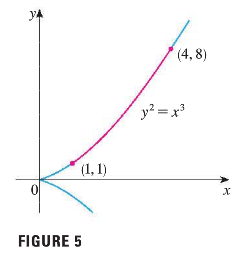
\includegraphics[scale=0.5]{8-1pic4.png}
  
  \vspace{3in}
  
  \underline{Example 2}: Find the length of the arc of the parabola $y^2=x$ from $(0,0)$ to $(1,1)$.\\
  \indent\\
  
  \vspace{4in}
  
  \section*{The Arc Length Function}
  
  We will find it useful to have a function that measures the arc length of a curve from a particular starting point to any other point on the curve. Thus if a smooth curve $C$ has the equation $y=f(x), a\leq x\leq b$, let $s(x)$ be the distance along $C$ from the initial point $P_0(a,f(a))$ to the point $Q(x,f(x))$. Then $s$ is a function, called the \underline{\hspace{0.5in}} \underline{\hspace{1in}} \underline{\hspace{1.25in}}, and from the above definition,\\
  
  \[s(x) = \hspace{3in}\]
  \indent\\
  \indent
  
  \underline{Example 3}: Find the arc length function for the curve $y=x^2-\ds\frac{1}{8}\ln x$ taking $P_0(1,1)$ as the\\
  \hspace{0.81in} starting point.\\
  \indent
  
  \vspace{3.8in}
  
  \[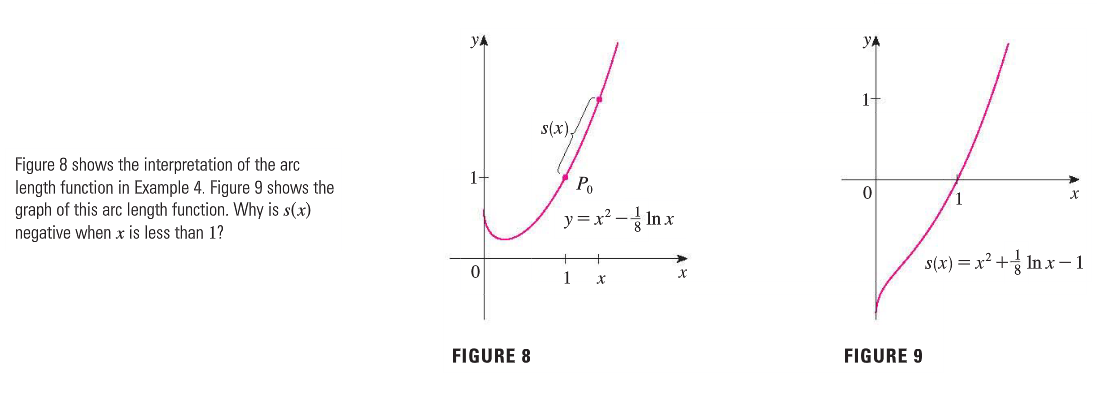
\includegraphics[scale=0.45]{8-1pic5.png}\]



%\fbox{
%  \parbox{\textwidth}{
%  \vspace{5pt}

















%----------------------------------------------------------------------------------------

\end{document}